\documentclass[11pt]{article}

\usepackage[margin=1in]{geometry}
\usepackage{amsmath,amssymb}
\usepackage{booktabs}
\usepackage{graphicx}
\usepackage{caption}
\usepackage{subcaption}
\usepackage{fancyhdr}
\usepackage{xcolor}
\usepackage[hidelinks,colorlinks=true,linkcolor=blue!60!black,citecolor=blue!60!black,urlcolor=blue!60!black]{hyperref}

\graphicspath{{figures/}}

\pagestyle{fancy}
\fancyhf{}
\lhead{\small Anastasiia Rekovets}
\rhead{\small NYU Stern -- Junior Research Scientist Sample Tasks}
\rfoot{\small \thepage}
\renewcommand{\headrulewidth}{0.4pt}

\captionsetup{font=small,labelfont=bf}
\setlength{\parskip}{0.4em}

\newcommand{\code}[1]{\texttt{\small #1}}

\title{\vspace{-2em}\textbf{Junior Research Scientist Sample Tasks}\\[0.4em]
       \large NYU Stern School of Business}
\author{Anastasiia Rekovets}
\date{June 2026}

\begin{document}

\maketitle
\thispagestyle{empty}

\begin{abstract}
\noindent
This report summarises a two-part analysis. Part~1 uses the Expedia
\emph{Personalizing Hotel Searches} dataset (9.9M impressions across 399,344
search sessions) to estimate the causal effect of hotel prices on click and
booking probability, using OLS, within-session fixed effects, IV/2SLS and
double/debiased machine learning, followed by a sequential search model
(Ursu, Seiler and Honka, 2024) estimated by simulated maximum likelihood.
The preferred within-session estimate implies that a 10\% price increase
lowers click probability by roughly 0.28 percentage points (about 6\% of the
baseline click rate). The IV specification is reported as a diagnostic rather
than a preferred estimate: its first stage is strong, but the correction runs
in the opposite direction to what quality-driven endogeneity predicts, which
is itself evidence against the exclusion restriction. Part~2 replicates the
$N=3$ algorithmic pricing setting of Liu et al.\ (2026) using Q-learning over
a restricted rule set. The headline collusion index replicates exactly
($\Delta = 1.000$), but the paper's state-robustness check does \emph{not}
replicate (28\% of runs versus 100\% reported), which qualifies the
interpretation of the headline result.

\vspace{1em}
\noindent\textbf{Reproducibility.} Every number, table and figure in this
report is taken directly from the saved outputs of the two accompanying
notebooks. Table and figure sources are named in the notes to each exhibit.

\vspace{0.5em}
\noindent\textbf{AI tool usage.} Claude was used as a coding assistant for
syntax and debugging.
\end{abstract}

\clearpage
\tableofcontents
\clearpage

%=============================================================================
\section{Part 1: Hotel Search -- Data Analysis and Structural Estimation}
%=============================================================================

\subsection{Data Assessment and Summary Statistics (Tasks 1 \& 2)}

The analysis uses the Expedia \emph{Personalizing Hotel Searches} dataset
(Expedia, Inc., 2013), processed out-of-core with \code{polars}. The training
file contains 9,917,530 hotel--search impressions across 399,344 unique search
sessions and 136,886 unique properties, covering 1 November 2012 to 30 June
2013, with an average of 24.8 hotels listed per search. The outcomes are
\code{click\_bool} (4.47\% overall, 443,672 clicks) and \code{booking\_bool}
(2.79\%, 276,593 bookings). No booking occurs without a click, and
$P(\text{book} \mid \text{click}) = 62.34\%$.

\paragraph{Assessment.} The scale of the data and the real financial stakes
make it well suited to studying price--demand relationships. Its central
strength is the \code{random\_bool = 1} subsample (2,939,652 rows, 29.6\% of
the data), in which hotels are displayed in random order. This provides
strictly exogenous variation in display position and is the basis for the
preferred specifications below.

Three limitations deserve emphasis. First, missingness is severe in exactly
the variables that would be most valuable: \code{gross\_bookings\_usd} is
97.2\% missing (precluding revenue-weighted analysis), the
\code{visitor\_hist\_*} fields are 94.9\% missing (individual price
sensitivity is unobserved), and the competitor price fields are 55--98\%
missing, reflecting structural absence -- the hotel is not listed on that OTA
-- rather than random non-response. Second, the platform sample is selected:
these are Expedia searches, not the travel market. Third, and most important
for interpretation, the random-order subsample behaves oddly. Its click rate
is \emph{higher} than in ranked sessions (4.66\% vs 4.40\%), while its booking
rate is roughly seven times \emph{lower} (0.54\% vs 3.74\%). A pure position
effect would not produce a seven-fold booking gap alongside a higher click
rate. The more cautious reading is that random-order clicks partly reflect
browsing curiosity rather than purchase intent, and that random-order sessions
may not be a clean random draw from the same population. Estimates identified
off this subsample (M3r, M4, M6 below) should be read with that in mind,
particularly for bookings.

\begin{table}[htbp]
  \centering
  \caption{Summary Statistics for Continuous Variables}
  \label{tab:summary}
  \small
  \begin{tabular}{lrrrrrrrr}
    \toprule
    Variable & $N$ & Mean & Std & Min & P25 & P50 & P75 & Max \\
    \midrule
    \code{price\_usd}                 & 9,917,530 & 241.78 & 14,341.81 & 0.00 & 85.00 & 122.07 & 185.00 & 19,726,328 \\
    \code{log\_price\_usd}            & 9,917,476 & 4.85 & 0.62 & $-4.61$ & 4.44 & 4.80 & 5.22 & 16.80 \\
    \code{prop\_log\_historical\_price} & 9,917,530 & 4.32 & 1.84 & 0.00 & 4.44 & 4.91 & 5.31 & 6.21 \\
    \code{prop\_starrating}           & 9,917,530 & 3.18 & 1.05 & 0.00 & 3.00 & 3.00 & 4.00 & 5.00 \\
    \code{prop\_review\_score}        & 9,902,900 & 3.78 & 1.05 & 0.00 & 3.50 & 4.00 & 4.50 & 5.00 \\
    \code{prop\_location\_score1}     & 9,917,530 & 2.88 & 1.53 & 0.00 & 1.79 & 2.77 & 4.04 & 6.98 \\
    \code{srch\_length\_of\_stay}     & 9,917,530 & 2.39 & 2.07 & 1.00 & 1.00 & 2.00 & 3.00 & 59.00 \\
    \code{srch\_booking\_window}      & 9,917,530 & 37.62 & 52.11 & 0.00 & 4.00 & 17.00 & 49.00 & 498.00 \\
    \code{position}                   & 9,917,530 & 16.87 & 10.43 & 1.00 & 8.00 & 16.00 & 26.00 & 40.00 \\
    \bottomrule
  \end{tabular}
  \vspace{0.6ex}
  \begin{minipage}{0.95\textwidth}
  \footnotesize \textit{Notes:} Unit of observation is a hotel--search-session
  impression. \code{price\_usd} is extremely right-skewed (54 rows are exactly
  zero and 5,707 rows exceed \$5,000; both are almost certainly data errors),
  which is why all models use \code{log\_price\_usd}. The 54 zero-price rows
  are set to null and excluded from every regression. A further 1,430,427 rows
  have \code{prop\_log\_historical\_price} $= 0$, a missing-value sentinel
  implying a \$1 historical rate; these are dropped where that variable is used
  as a regressor or instrument. Source: notebook Part~1, cell~7.
  \end{minipage}
\end{table}

\begin{table}[htbp]
  \centering
  \caption{Click and Booking Rates by Log-Price Decile}
  \label{tab:deciles}
  \small
  \begin{tabular}{lrrrr}
    \toprule
    Decile & $N$ & Median price (\$) & Click rate (\%) & Booking rate (\%) \\
    \midrule
    1 (cheapest)   &   995,902 &  51.00 & 4.37 & 2.81 \\
    2              &   987,605 &  70.00 & 4.64 & 3.13 \\
    3              &   991,776 &  85.00 & 4.94 & \textbf{3.36} \\
    4              &   993,419 &  99.00 & \textbf{4.98} & 3.28 \\
    5              &   990,038 & 114.76 & 4.89 & 3.19 \\
    6              & 1,002,811 & 131.06 & 4.83 & 3.07 \\
    7              & 1,049,587 & 155.00 & 4.58 & 2.79 \\
    8              &   928,649 & 186.77 & 4.37 & 2.56 \\
    9              &   985,963 & 234.11 & 4.05 & 2.26 \\
    10 (most exp.) &   991,726 & 356.00 & 3.07 & 1.41 \\
    \bottomrule
  \end{tabular}
  \vspace{0.6ex}
  \begin{minipage}{0.9\textwidth}
  \footnotesize \textit{Notes:} Source: notebook Part~1, cell~12. Demand is
  \emph{not} monotonically decreasing in price. Both click and booking rates
  rise from decile 1 to a peak at decile 3--4 (booking 3.36\% at a median of
  \$85) before declining steadily; the fall is steepest above decile 8. The
  upturn at the bottom is economically meaningful rather than noise: the very
  cheapest listings attract fewer clicks than mid-priced ones, consistent with
  low price acting as a negative quality signal. A purely monotone reading of
  the raw decile gradient would miss this.
  \end{minipage}
\end{table}

Quality signals also shift baseline rates substantially. Click rates by star
rating are non-monotone and peak at four stars (5.39\%), above both three-star
(4.38\%) and five-star (4.59\%) properties; unrated and one-star properties sit
lowest (2.90\% and 2.80\%). The largest single gap in the data comes from
promotions: properties with an active promotion are clicked 6.04\% of the time
versus 4.04\% without, and booked 3.92\% versus 2.48\%.

\subsection{Visualising Price Effects (Task 3)}

Visual analysis isolates the endogeneity of display position. Figure~\ref{fig:deciles}a
shows click and booking rates across raw price deciles pooled over all sessions.
Figure~\ref{fig:deciles}b restricts to random-order sessions, where the gradient
flattens substantially. The difference is direct evidence that Expedia's ranking
algorithm confounds the price effect by systematically placing cheaper hotels
higher on the page.

\begin{figure}[htbp]
  \centering
  \begin{subfigure}{0.49\textwidth}
    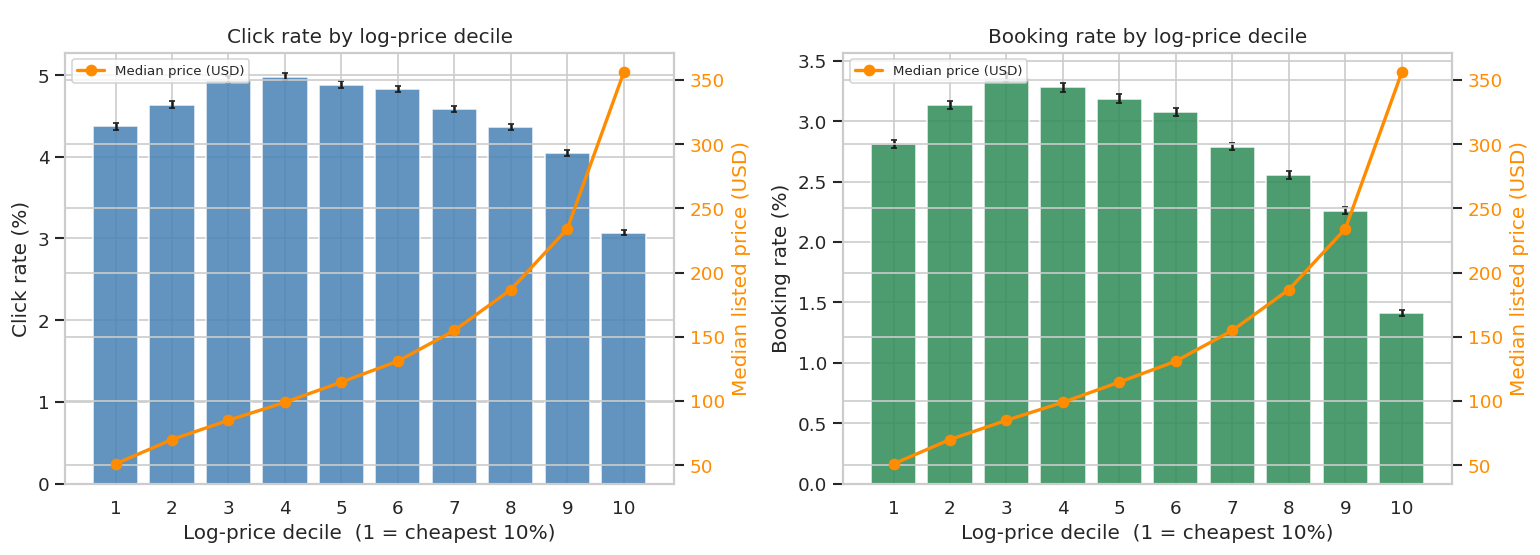
\includegraphics[width=\linewidth]{fig1a_decile_all_sessions.png}
    \caption{All sessions (position endogenous)}
  \end{subfigure}\hfill
  \begin{subfigure}{0.49\textwidth}
    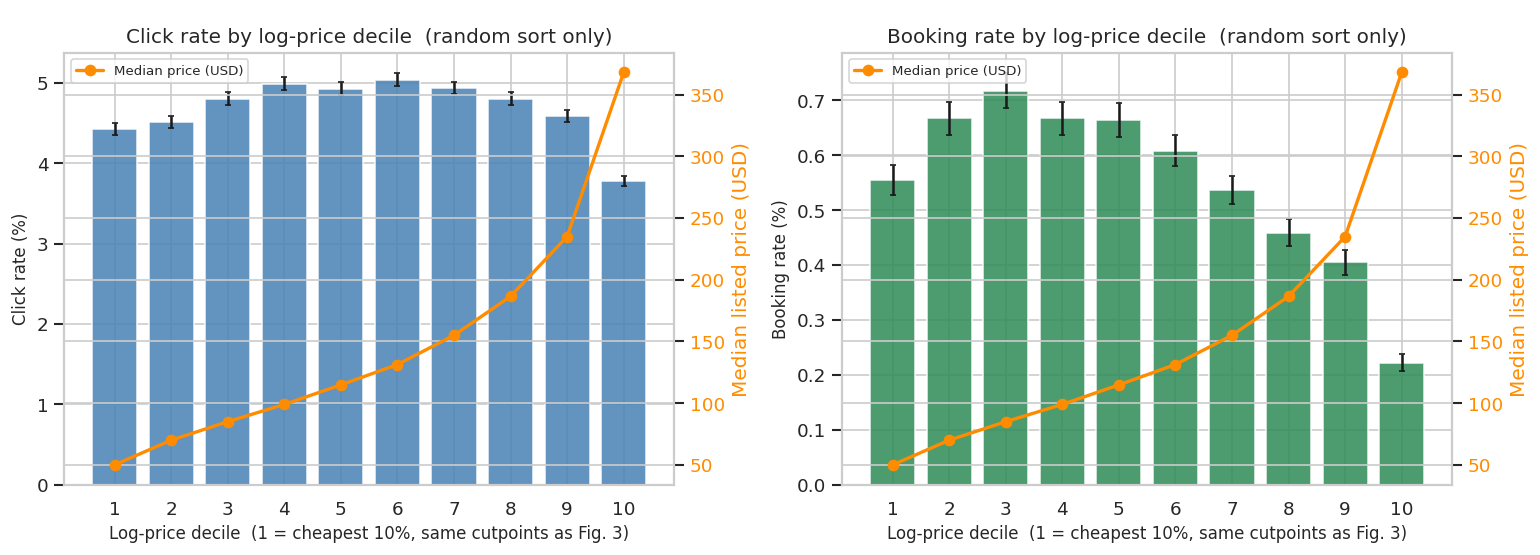
\includegraphics[width=\linewidth]{fig1b_decile_random.png}
    \caption{Random-order sessions (\code{random\_bool}$=1$)}
  \end{subfigure}
  \caption{Click and booking rates by log-price decile. The flattening in (b)
  isolates the position confound. Source: notebook Part~1, cells~12--13.}
  \label{fig:deciles}
\end{figure}

The sharpest descriptive evidence comes from comparing a hotel to the
alternatives shown in the \emph{same} session, which absorbs all
session-level confounders. Figure~\ref{fig:rank} plots outcomes against
within-search price rank in random-order sessions: the cheapest hotel in a
session is clicked 8.67\% of the time, falling to 6.22\% at rank 5 and 4.62\%
at rank 10 -- a 1.39$\times$ ratio between ranks 1 and 5, with a corresponding
1.26$\times$ ratio for bookings.

\begin{figure}[htbp]
  \centering
  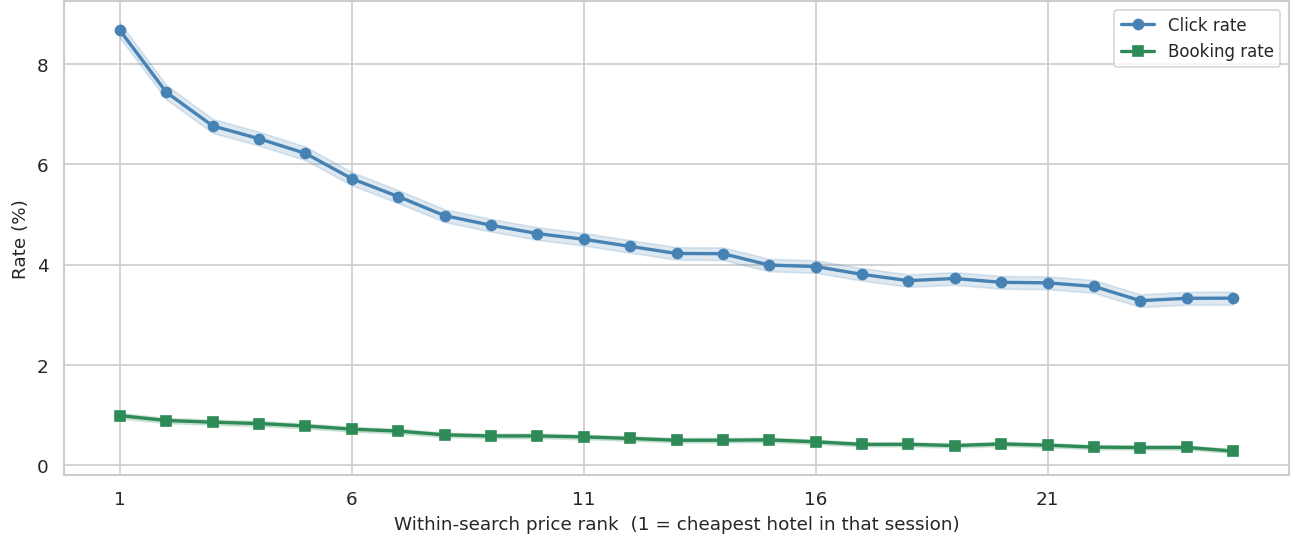
\includegraphics[width=0.62\textwidth]{fig2_within_search_rank.png}
  \caption{Outcomes by within-search price rank (\code{random\_bool}$=1$).
  Source: notebook Part~1, cell~14.}
  \label{fig:rank}
\end{figure}

Figure~\ref{fig:dens} shows that booked hotels concentrate at lower prices and
that price sensitivity persists strictly within star-rating tiers, so the
gradient is not simply quality sorting. A useful diagnostic sits in the same
cell: among ranked sessions, clicked hotels are on average \$12.0 cheaper than
unclicked ones, but in random-order sessions the gap narrows to \$5.6 --
again indicating that a large share of the raw price--click association is a
display artefact.

\begin{figure}[htbp]
  \centering
  \begin{subfigure}{0.49\textwidth}
    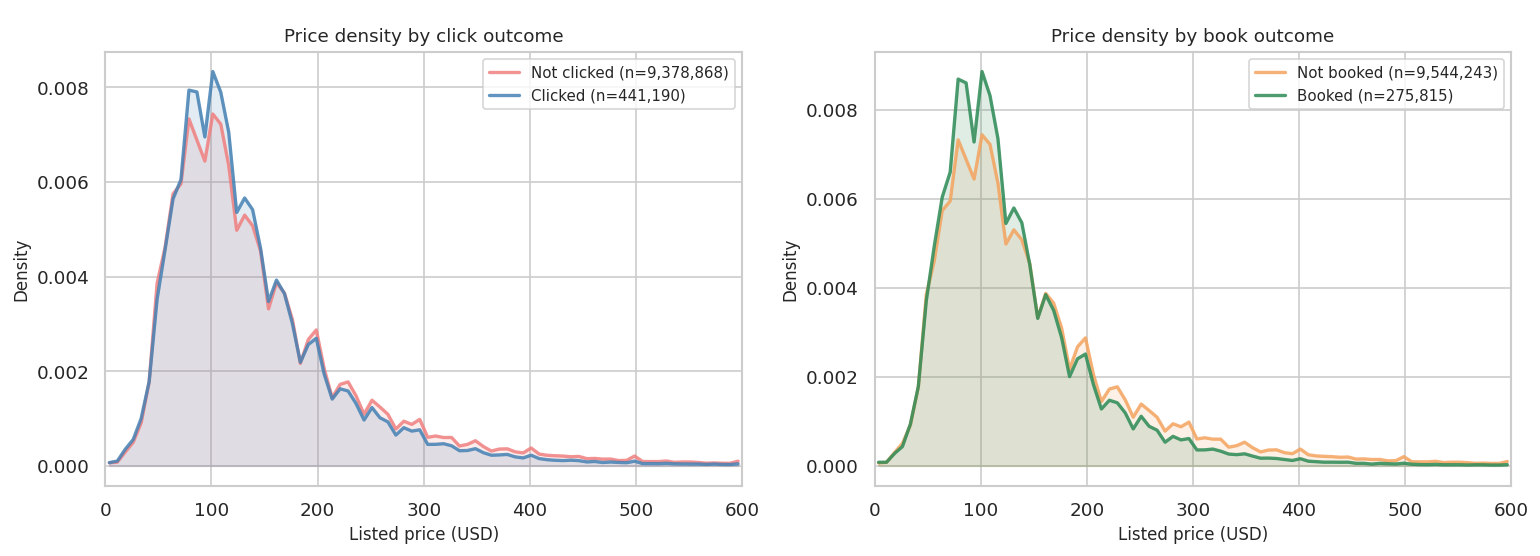
\includegraphics[width=\linewidth]{fig3a_price_density.png}
    \caption{Price density by outcome}
  \end{subfigure}\hfill
  \begin{subfigure}{0.49\textwidth}
    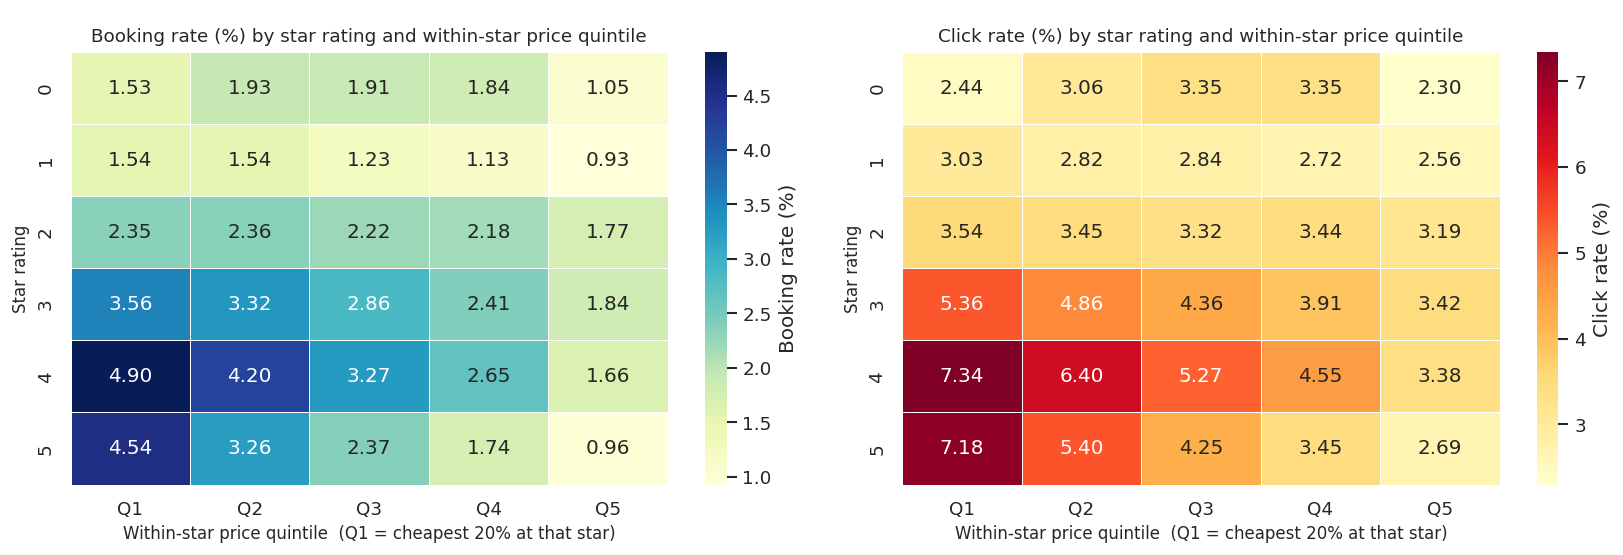
\includegraphics[width=\linewidth]{fig3b_star_price_quintile.png}
    \caption{Booking rate by star rating and within-star price quintile}
  \end{subfigure}
  \caption{Price distributions and quality--price interactions. Source:
  notebook Part~1, cells~15--16.}
  \label{fig:dens}
\end{figure}

\subsection{Causal Impact of Hotel Prices: Regression Framework (Task 4)}

To separate the causal price effect from unobserved quality and display
position, I estimate a series of linear probability models,
%
\begin{equation}
y_{ij} = \alpha + \beta \log p_{ij} + \boldsymbol{\gamma}' \mathbf{X}_{ij}
         + \delta \, \text{position}_{ij} + \varepsilon_{ij},
\end{equation}
%
where $\beta$ is a semi-elasticity: a 1\% price increase changes the outcome
probability by $\beta/100$ percentage points. Eight specifications are
estimated:

\begin{itemize}\itemsep2pt
  \item \textbf{M1--M3 (OLS).} Progressively add hotel quality controls and
        display position, on a 2M-row sample.
  \item \textbf{M3r.} M3 re-estimated on random-order sessions only. Comparing
        M3 to M3r isolates the \emph{sample} restriction.
  \item \textbf{M3\_IV.} M3 re-estimated on the exact 500k rows used for M5, so
        that the M3\_IV$\rightarrow$M5 comparison is a clean OLS-versus-IV
        contrast unconfounded by sample composition.
  \item \textbf{M4 (within-session FE).} Restricted to \code{random\_bool}$=1$
        and demeaned within \code{srch\_id} by the Frisch--Waugh--Lovell
        theorem, absorbing every search-level unobservable. SEs clustered on
        session.
  \item \textbf{M5 (IV/2SLS).} Instruments price with
        \code{prop\_log\_historical\_price}.
  \item \textbf{M6 (DDML).} Partially linear regression with histogram
        gradient-boosted nuisance functions and cross-fitting, relaxing
        linearity in controls.
\end{itemize}

\begin{table}[htbp]
  \centering
  \caption{Price Coefficient Estimates Across Specifications}
  \label{tab:regression}
  \small
  \begin{tabular}{llrcc}
    \toprule
    Model & Estimator & $N$ & Click coef. & Booking coef. \\
    \midrule
    M1: Bivariate OLS      & OLS, HC1              & 2,000,000 & $-0.0063^{***}$ & $-0.0071^{***}$ \\
                           &                       &           & $(0.0002)$ & $(0.0002)$ \\
    M2: $+$Controls        & OLS, HC1              & 2,000,000 & $-0.0143^{***}$ & $-0.0116^{***}$ \\
                           &                       &           & $(0.0003)$ & $(0.0002)$ \\
    M3: $+$Position        & OLS, HC1              & 2,000,000 & $-0.0148^{***}$ & $-0.0120^{***}$ \\
                           &                       &           & $(0.0003)$ & $(0.0002)$ \\
    M3r: $+$Pos.\ (random) & OLS, HC1 (random)     & 2,933,760 & $-0.0114^{***}$ & $-0.0025^{***}$ \\
                           &                       &           & $(0.0002)$ & $(0.0001)$ \\
    M3\_IV: $+$Pos.\ (IV sample) & OLS, HC1 (IV sample) & 500,000 & $-0.0145^{***}$ & $-0.0118^{***}$ \\
                           &                       &           & $(0.0005)$ & $(0.0004)$ \\
    \textbf{M4: Within-session FE} & FE, clustered SE & 2,933,760 & $\mathbf{-0.0298^{***}}$ & $\mathbf{-0.0049^{***}}$ \\
                           &                       &           & $(0.0004)$ & $(0.0001)$ \\
    M5: IV / 2SLS          & IV2SLS, robust SE     & 500,000   & $-0.0074^{***}$ & $-0.0092^{***}$ \\
                           &                       &           & $(0.0008)$ & $(0.0006)$ \\
    M6: DDML (HGBR)        & DDML PLR, cross-fit   & 150,000   & $-0.0134^{***}$ & $-0.0024^{***}$ \\
                           &                       &           & $(0.0011)$ & $(0.0003)$ \\
    \bottomrule
  \end{tabular}
  \vspace{0.6ex}
  \begin{minipage}{0.95\textwidth}
  \footnotesize \textit{Notes:} Source: notebook Part~1, cell~25. Standard
  errors in parentheses. $^{***}p<0.01$, $^{**}p<0.05$, $^{*}p<0.10$. All
  coefficients are semi-elasticities on log price, including M4's
  within-session demeaned log price, so magnitudes are directly comparable
  across rows. Every coefficient in the table, M6's booking estimate included,
  is significant at the 1\% level. The preferred specification is M4.
  \end{minipage}
\end{table}

\begin{figure}[htbp]
  \centering
  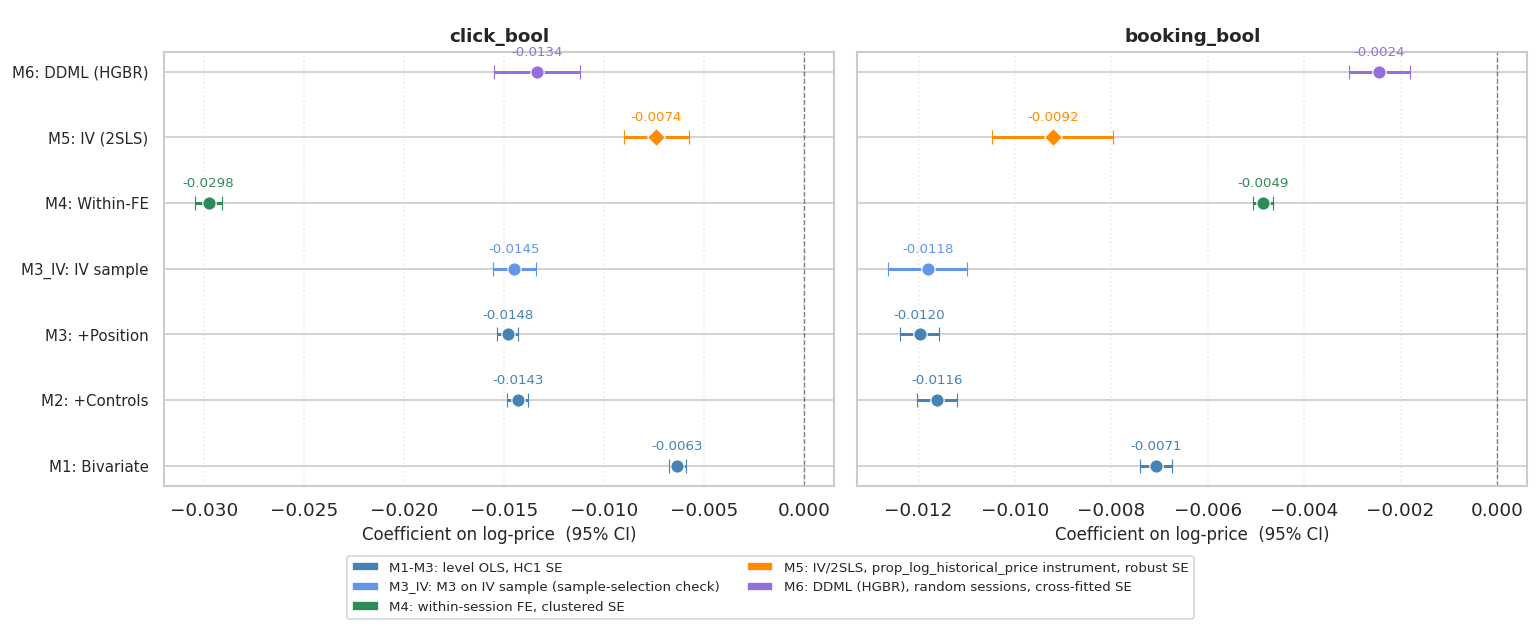
\includegraphics[width=\textwidth]{fig4_coefficient_plot.png}
  \caption{Price coefficient semi-elasticities across specifications (95\% CI).
  Source: notebook Part~1, cell~24.}
  \label{fig:coefplot}
\end{figure}

\paragraph{Interpretation and magnitudes.} Price reduces demand in every
specification. Taking M4 as the preferred estimate, a 10\% price increase
($\Delta \log p = 0.0953$) lowers click probability by
$0.0298 \times 0.0953 = 0.28$ percentage points. Against the 4.66\% baseline
click rate in random-order sessions, that is a decline of about 6\% in
relative terms. The corresponding booking effect is
$0.0049 \times 0.0953 = 0.047$ percentage points, roughly 8.6\% of the 0.54\%
random-order booking base rate. The much smaller absolute booking coefficient
therefore does not indicate weaker price sensitivity for bookings; it reflects
the very low booking base rate in this subsample, and the two relative
magnitudes are broadly comparable.

The decomposition built into the table is worth reading directly. Moving from
M3 ($-0.0148$) to M3r ($-0.0114$) is the pure \emph{sample} effect of
restricting to random-order sessions; moving from M3r to M4 ($-0.0298$) is the
pure \emph{estimator} effect of within-session demeaning. The within-session
estimate is roughly twice the pooled OLS estimate, which is what we expect if
session-level unobservables (destination, dates, party composition, and the
overall price level of the choice set) mask price sensitivity in the pooled
data.

\paragraph{The IV specification is a diagnostic, not a preferred estimate.}
The first stage is strong on conventional criteria: the instrument enters with
a coefficient of $0.8901$ (SE $0.0017$), the partial $F$-statistic is
261,009.8, and the Shea partial $R^2$ is $0.43078$. Weak-instrument bias is
therefore not the binding concern here, and it would be wrong to dismiss M5 on
those grounds.

The binding concern is the exclusion restriction, and the estimates themselves
supply evidence against it. The instrument is the same hotel's own historical
Expedia rate, which plausibly proxies for persistent unobserved
quality and amenities that enter demand directly. The near-unit pass-through
from historical to current price is exactly what a persistent, quality-driven
price level would generate, so the strong first stage is as much a warning as
a reassurance.

The direction of the correction makes this concrete. On the identical 500,000
rows, OLS gives $-0.0145$ (click) and $-0.0118$ (booking), while 2SLS gives
$-0.0074$ and $-0.0092$: the IV estimates are \emph{less} negative than OLS.
The standard quality-endogeneity story predicts the opposite. If expensive
hotels are systematically better in ways we do not observe, and quality raises
demand, then OLS is biased toward zero and a valid instrument should push the
estimate \emph{more} negative. Obtaining a correction in the wrong direction is
the signature of an instrument that carries the very quality signal it was
meant to purge. The Wu--Hausman tests reject exogeneity (click statistic
124.27, booking 26.29, both $p<0.0001$), but at $N=500{,}000$ that test rejects
on economically trivial differences and does not rescue the design. M5 is
reported here for completeness and as evidence about the instrument; it is not
used as a causal estimate.

\subsection{Sequential Search Model (Task 5)}

Following Ursu, Seiler and Honka (2024), consumer utility for hotel $j$ is
%
\begin{equation}
u_{ij} = \delta_{ij} + \mu_{ij} + \varepsilon_{ij},
\qquad \delta_{ij} = \mathbf{X}'_{ij}\boldsymbol{\beta},
\end{equation}
%
where $\mu_{ij}$ and $\varepsilon_{ij}$ are standard normal pre- and
post-search shocks. The reservation utility equates the marginal gain from
searching with its cost, $z_{ij} = \delta_{ij} + \mu_{ij} + m(c_{ij})$, and
search costs are position-dependent,
$c_{ij} = \exp(\gamma_0 + \gamma_1 \cdot \text{position}_{ij})$.

The model is estimated by simulated maximum likelihood on 2,000 random-order
sessions with $D = 300$ draws, drawn from the 38,937 sessions with at least one
click and between 2 and 20 listings. Of the estimation sample, 276 sessions
(13.8\%) end in a booking and 1,724 (86.2\%) in no purchase. Standard errors
come from a subsampled bootstrap (Politis--Romano) with $B = 100$ replicates of
$m = 500$ sessions; 2 replicates failed to converge.

\begin{table}[htbp]
  \centering
  \caption{Sequential Search Model Estimates}
  \label{tab:structural}
  \small
  \begin{tabular}{lrrrr}
    \toprule
    Parameter & Estimate & Approx.\ SE & $t$-stat & 95\% CI \\
    \midrule
    $\beta_{\text{price}}$ (log price)      & $-0.6454$ & 0.0098 & $-66.17$ & $[-0.665,\,-0.626]$ \\
    $\beta_{\text{star}}$ (star rating)     & $+0.0614$ & 0.0006 & $96.16$  & $[+0.060,\,+0.063]$ \\
    $\beta_{\text{review}}$ (review score)  & $+0.1254$ & 0.0019 & $66.06$  & $[+0.122,\,+0.129]$ \\
    $\beta_{\text{location}}$ (location score 1) & $-0.0560$ & 0.0006 & $-95.17$ & $[-0.057,\,-0.055]$ \\
    $\beta_{\text{brand}}$ (brand hotel)    & $+0.0216$ & 0.0002 & $127.55$ & $[+0.021,\,+0.022]$ \\
    $\beta_{\text{promo}}$ (promotion flag) & $+0.0300$ & 0.0002 & $136.07$ & $[+0.030,\,+0.030]$ \\
    $\beta_0$ (base hotel intercept)        & $-0.6023$ & 0.0085 & $-71.14$ & $[-0.619,\,-0.586]$ \\
    $\gamma_0$ (log baseline search cost)   & $-1.2547$ & 0.0222 & $-56.39$ & $[-1.298,\,-1.211]$ \\
    $\gamma_1$ (position effect on cost)    & $+0.0457$ & 0.0007 & $62.42$  & $[+0.044,\,+0.047]$ \\
    \bottomrule
  \end{tabular}
  \vspace{0.6ex}
  \begin{minipage}{0.95\textwidth}
  \footnotesize \textit{Notes:} Source: notebook Part~1, cell~32. $N = 2{,}000$
  sessions, $D = 300$ draws, subsampled bootstrap $B = 100$. $\sigma_\mu =
  \sigma_\varepsilon = 1$ is a normalisation, so coefficient magnitudes are
  interpretable only relative to one another. The reported standard errors
  should be treated as indicative rather than exact; see the discussion of
  their plausibility below.
  \end{minipage}
\end{table}

\paragraph{Results.} The structural parameters separate preferences from search
frictions. Expected utility falls with price ($\hat\beta_{\text{price}} =
-0.645$), and star rating, review score, brand and promotion all enter
positively. Since the scale is normalised, magnitudes are meaningful only in
relative terms: one additional star is worth about $0.095$ log-price units and
a one-unit increase in review score about $0.194$ log-price units. The negative
coefficient on \code{prop\_location\_score1} is contrary to expectation and is
best read as that variable proxying for something else once price and the other
quality measures are conditioned on, rather than as consumers disliking good
locations.

Search costs rise with depth on the page ($\hat\gamma_1 = +0.046 > 0$),
implying about 4.7\% higher cost per position and making position 20 roughly
$2.38\times$ as costly to reach as position 1. In levels, the implied cost
rises from $0.299$ at position 1 to $0.712$ at position 20. Forward-simulating
the search process at $\hat\theta$ reproduces the observed behaviour reasonably
well: 1.03 model clicks per session against 1.10 observed, with a click
gradient of 13.4\%, 8.7\%, 5.0\%, 3.1\% across position buckets 1--5, 6--10,
11--15 and 16--20, against observed values of 15.8\%, 8.4\%, 4.5\% and 2.7\%.
Fit deteriorates in the 21--40 bucket (2.0\% model versus 3.8\% observed).

\paragraph{Limitations.} Four caveats apply, and the first two are substantial.

First, the reported standard errors are implausibly small. $t$-statistics
between 62 and 136 on a 2,000-session simulated likelihood with $D = 300$ are
not credible; they almost certainly reflect the subsampling rescaling in the
bootstrap rather than genuine precision. The point estimates should be taken as
the informative output of this exercise and the standard errors treated as a
known open problem, to be replaced by a properly rescaled subsampling variance
or a numerical Hessian before any inference is drawn. I flag this rather than
report inference I do not believe.

Second, 7.6\% of sessions sit at the $10^{-10}$ likelihood floor, meaning the
log-likelihood is partly driven by the floor rather than by the model; $D$
should be raised until that share is negligible.

Third, identification of the search-order rule is weak: sessions average only
1.11 clicks, so most of the information comes from stopping and choice rather
than from the order in which alternatives are inspected. Relatedly, the data
contain no intra-session timestamps, so the likelihood assumes consumers search
in top-to-bottom display order.

Fourth, $\sigma_\varepsilon = 1$ is a normalisation, so search costs cannot be
monetised, and $D = 300$ with $N = 2{,}000$ was chosen for speed; production
work would use $D \geq 500$ and the full session set.

Finally, the structural and reduced-form estimates are not directly comparable
in magnitude. $\beta_{\text{price}}$ is on a utility scale while the Task~4
coefficients are probability-scale semi-elasticities; they agree in sign, and
the value the structural model adds is separating the preference channel from
the search-friction channel that the reduced form bundles together.

%=============================================================================
\section{Part 2: Algorithmic Pricing -- Q-Learning Simulation}
%=============================================================================

\subsection{Action Space Bounds \& Setup (Task Q1)}

The simulation restricts algorithmic prices to $m = 10$ grid points bounded by
the Bertrand--Nash price $p^N$ and the monopoly price $p^M$. For a logit demand
model with $N = 3$, $a_i = 2.0$, $c = 1.0$, $\mu = 0.25$, numerically solving
the respective first-order conditions yields $p^N = 1.3702$ and $p^M = 2.0000$,
with per-seller profits $r^N = 0.1202$ and $r^M = 0.2500$. With the extension
factor $\xi = 0.1429$, the resulting grid runs from $1.2802$ to $2.0900$ in
steps of $0.0900$, matching the $p_{\min} = 1.28$ and $p_{\max} = 2.09$
reported in Table 2 of Liu et al.\ (2026). Note that $p^M$ falls at grid index
8 of 10 rather than at the top of the grid.

Three symmetric sellers use Q-learning to select among rules
$\mathcal{A} = \{\text{Undercut}, \text{Match}, \text{Above}\}$ based on the
minimum competitor price $s_t$, committing to the chosen rule for $K = 30$
inner periods before updating Q-values via the standard Bellman equation.

\subsection{Simulation Results}

\begin{table}[htbp]
  \centering
  \caption{Replication Results: $N = 3$, 3-Rule Set}
  \label{tab:replication}
  \small
  \begin{tabular}{lcc}
    \toprule
    Metric & Computed ($B = 50$ seeds) & Paper (Table 2) \\
    \midrule
    $\Delta$ (mean $\pm$ std)      & $1.000 \pm 0.000$ & $1.000 \pm 0.000$ \\
    Avg.\ low price                & $2.000 \pm 0.000$ & $2.00 \pm 0.00$ \\
    Converged (\%)                 & 100\% & 100\% \\
    Nash equilibrium (\%)          & 100\% & 100\% \\
    \textbf{State robust (\%)}     & \textbf{28\%} & \textbf{100\%} \\
    Convergence episodes (mean)    & 720,439 & n/a \\
    \bottomrule
  \end{tabular}
  \vspace{0.6ex}
  \begin{minipage}{0.9\textwidth}
  \footnotesize \textit{Notes:} Source: notebook Part~2, cell~8. $B = 50$
  independent seeds, burn-in of 1,000 episodes. Per-seller $\Delta$ values are
  all $1.000 \pm 0.000$, confirming a symmetric equilibrium. The Nash check is a
  one-shot deviation test, not full subgame perfection.
  \end{minipage}
\end{table}

The headline result replicates exactly. Across 50 independent seeds the market
locks at $p^M = 2.00$ with zero price dispersion, giving a collusion index of
$\Delta = 1.00$, and every run converges and passes the one-shot Nash
deviation check.

\paragraph{One check does not replicate.} State robustness holds in only 28\% of
runs, against the 100\% reported in the paper. This is the most informative
result in Part~2 and it should not be folded into the passing rows. Converged
policies attain the collusive price but are, in most runs, not robust to
perturbing the state: the equilibrium is reached reliably yet supported
fragilely. The converged policy from run 1 illustrates the mechanism -- all three
sellers play \emph{Above} across most of the state space and switch to
\emph{Match} only near $p^M$, so the Q-values that sustain cooperation are
sharply defined at the collusive state and thin elsewhere. Whether the gap
reflects a difference in how robustness is defined, the restriction to $B = 50$
seeds, or a genuine failure of the paper's claim cannot be settled from this
replication alone, and is the first thing I would take up with the authors.

\begin{figure}[htbp]
  \centering
  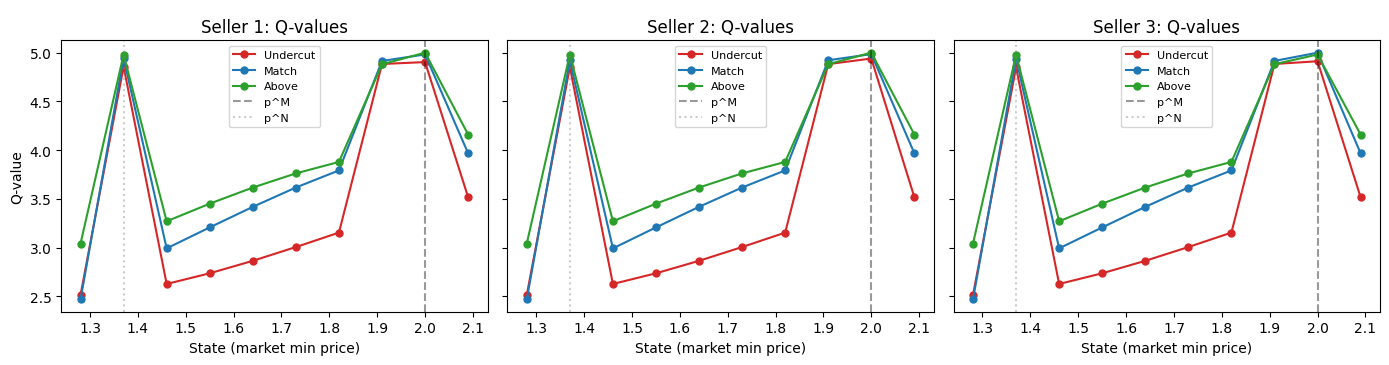
\includegraphics[width=\textwidth]{fig5_qvalues.png}
  \caption{Converged Q-values by seller. Vertical dashed line $= p^M$; dotted
  $= p^N$. Source: notebook Part~2, cell~8.}
  \label{fig:qvalues}
\end{figure}

\subsection{Drivers of High Collusion (Task Q2)}

The replication yields $\Delta = 1.00$ at $N = 3$, well above the
$\Delta \approx 0.85$ observed in unconstrained models such as Calvano et al.\
(2020). Three mechanisms explain the divergence, though the third is the one
that does most of the work.

\begin{enumerate}\itemsep3pt
  \item \textbf{Algorithmic commitment.} In Calvano et al., agents re-optimise
        period by period. Here they commit to a rule for $K = 30$ periods,
        which generates a slow-slide punishment for deviators that mimics a
        severe grim-trigger strategy and makes defection structurally
        unprofitable. The $K$-sweep in Figure~\ref{fig:ksweep} confirms the
        mechanism directly: $\Delta = 0.678$ at $K = 1$, and reaches 1.000 at
        $K = 5$ and every value above. The critical threshold is $K^* = 5$.
  \item \textbf{Compressed action space.} Unconstrained Q-learning at $N = 3$
        requires 50,625 cells per agent in Calvano et al. Restricting agents to
        three rules compresses the Q-table to 30 cells, a
        1,690$\times$ reduction that allows rapid and reliable convergence.
  \item \textbf{The rule set embeds coordination.} This point deserves more
        weight than a replication alone would give it. One of the three
        available actions is \emph{Match}, which sets a seller's price equal to
        its rival's. Coordination is therefore available as a primitive of the
        action space rather than something the algorithms must discover through
        trial and error, and \emph{Match} functions as a Schelling focal point.
        Finding $\Delta = 1.00$ under these conditions is a substantially weaker
        result than Calvano et al.'s finding of emergent collusion under
        unconstrained price competition, and the two numbers should not be read
        as measuring the same phenomenon. The fragility documented above
        reinforces this reading: the algorithms reach the collusive price
        easily because the rule set hands it to them, but the supporting
        Q-values are not robust.
\end{enumerate}

A robustness grid over the learning rate and exploration decay
($\alpha \in \{0.10, 0.15, 0.25\}$, $\beta \in \{5\times10^{-6},
1\times10^{-5}, 2\times10^{-5}\}$) yields $\Delta$ between $0.970$ and $1.000$,
so the headline result is not an artefact of the chosen hyperparameters.

\begin{figure}[htbp]
  \centering
  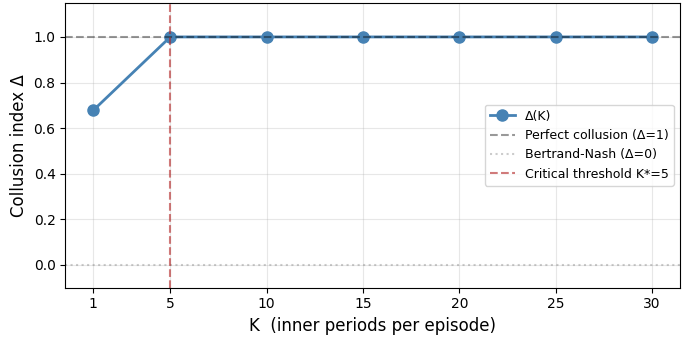
\includegraphics[width=0.62\textwidth]{fig6_ksweep.png}
  \caption{Collusion index $\Delta$ as a function of commitment length $K$.
  Source: notebook Part~2, cell~9.}
  \label{fig:ksweep}
\end{figure}

\subsection{Extension: Imperfect Competitor Monitoring (Task Q3)}

Liu et al.\ assume algorithms observe the minimum competitor price $s_t$
perfectly. Real pricing APIs are subject to latency and scraping error. I
propose replacing the perfect signal with an independent, noisy private draw:
%
\begin{equation}
\tilde{s}_{i,t} = \operatorname{clip}\!\left(s_t + \lfloor \varepsilon_{i,t}/\Delta p \rfloor,\ 0,\ m-1\right),
\qquad \varepsilon_{i,t} \overset{\text{iid}}{\sim} \mathcal{N}(0, \sigma^2).
\end{equation}

\paragraph{Predictions.} Noise introduces three failure modes: mistaken
punishments, missed defections, and asynchronous price wars. I predict $\Delta$
decays monotonically in $\sigma$. Crucially, high-$K$ commitment should
\emph{amplify} the cost of mistaken punishments -- a seller locked into a
punitive rule for 30 periods cannot correct a misreading -- reversing the
benefit documented in Mechanism 1 and generating an interior optimum for $K$.
The state-robustness failure reported above makes this prediction sharper: if
the converged policies are already fragile to state perturbation under a
perfect signal, then noise in the state signal should degrade them faster than
the $\Delta$ measure alone would suggest.

\paragraph{Policy relevance.} Article 6(1)(j) of the EU Digital Markets Act
mandates real-time price transparency. If lowering $\sigma$ raises $\Delta$,
mandatory transparency may inadvertently facilitate algorithmic collusion,
reversing the standard regulatory intuition. This is a testable implication of
the model rather than a finding of this report.

%=============================================================================
\clearpage
\section*{References}
\addcontentsline{toc}{section}{References}
%=============================================================================

\begin{description}\itemsep4pt
\item Calvano, E., Calzolari, G., Denicol\`o, V., and Pastorello, S. (2020).
      Artificial intelligence, algorithmic pricing, and collusion.
      \emph{American Economic Review}, 110(10):3267--3297.
\item Chernozhukov, V., Chetverikov, D., Demirer, M., Duflo, E., Hansen, C.,
      Newey, W., and Robins, J. (2018). Double/debiased machine learning for
      treatment and structural parameters. \emph{The Econometrics Journal},
      21(1):C1--C68.
\item Expedia, Inc. (2013). Personalize Expedia hotel searches. Kaggle
      Competition Dataset.
\item Liu, S., Wang, Q., and Ghose, A. (2026). Sophisticated learners, simple
      rules: The strategic selection of simple rules in algorithmic pricing.
      Working Paper 6810326, SSRN.
\item Politis, D. N., and Romano, J. P. (1994). Large sample confidence regions
      based on subsamples under minimal assumptions. \emph{Annals of
      Statistics}, 22(4):2031--2050.
\item Ursu, R., Seiler, S., and Honka, E. (2024). The sequential search model:
      A framework for empirical research. Working Paper 4236738, SSRN.
\end{description}

\end{document}
